This section introduces a potential implementation of solvers using the proposed
framework. The aim is to provide an overview of how meta-heuristic algorithms
can be developed utilizing the methods provided by the model API. To accomplish
this, we will start by describing a basic solver that utilizes heuristic
information for constructing solutions. Subsequently, we will demonstrate how
solvers for both~\acrshort{constructive-search} and~\acrshort{local-search}
methods can be implemented, using~\acrshort{beam-search}
and~\acrshort{iterated-local-search} meta-heuristics as illustrative examples.

\subsection{Heuristic Construction}
\label{subsec:heuristic-construction}

\Cref{lst:hc} describes a possible implementation of a
~\acrshort{meta-heuristic} solver that iteratively constructs a solution using
only heuristic information. This solver takes as input a~\texttt{Problem}
instance and returns a~\texttt{Solution}.

% Hill Climbing (algorithm2e pseudocode)

\KwIn{Solution ($s$), Objective Function ($f$)}
\KwOut{Solution ($s$)}

\SetKwFunction{Perturb}{\texttt{Perturb}}

\While{ \texttt{stopping criteria not met} }{
  $s'$ $\gets$ \Perturb{$s$}\;
  \If{$f(s') > f(s)$}{
    $s$ $\gets$ $s'$\;
  }
}
\Return{ $s$ }

This solver can be summarized as follows:

\begin{enumerate}
  \item \textbf{Initialization}: Initialize a new empty~\texttt{Solution}
        and select a~\texttt{Component} to be added heuristically.~(lines 2-3)
  \item \textbf{Construction}: Build the solution.~(lines 4-6)
        \begin{enumerate}
          \item If there is a component (\texttt{c}) available for addition to the
                current solution,~(\ie{},~\texttt{c} is not the~\texttt{None}
                sentinel value), proceed; otherwise stop.
          \item Add the selected component to the solution.
          \item Heuristically select a new component and repeat the process.
        \end{enumerate}
  \item \textbf{Termination} Return the final~\texttt{Solution}.~(line 7)
\end{enumerate}

As it can be observed this solver is simple and can be also used for easily
testing the model, given its only dependence on two basic methods:
the~\texttt{add} method for adding a component to the solution and the
~\texttt{heuristic\_add\_move} for selecting the next component to be added.


\subsection{Beam Search}
\label{subsec:beam-search-solver}
\begin{frame}{Problem}
  This problem entails the setup of scanning pipeline for books.

  \begin{itemize}
    \item There are libraries housing various books. Before any scanning can commence, each
          library needs to register for the scanning process. Once registered, each
          library is allowed to scan a certain number of books daily, until global deadline.
    \item Only one library can undergo the sign-up process at any given time.
    \item Each book, when scanned, contributes a specific score.
  \end{itemize}

\end{frame}

\begin{frame}{Example --- Book Scanning}
  \begin{figure}[h]
    \centering
    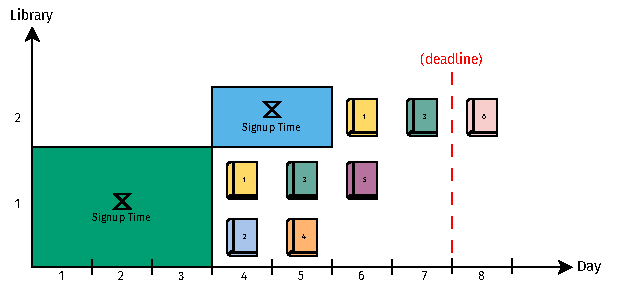
\includegraphics[width=0.8\textwidth,keepaspectratio]{../assets/bs/bs-example-slides.pdf}
    \caption{Book Scanning Example}
  \end{figure}

  \begin{table}[ht]
    \centering
    \begin{tabular}{ccccccc}
      \toprule
      \textbf{Book}  & 1 & 2 & 3 & 4 & 5 & 6 \\ \midrule
      \textbf{Score} & 3 & 1 & 5 & 4 & 7 & 1 \\
      \bottomrule
    \end{tabular}
    \caption{Book Scores}
  \end{table}
\end{frame}

\begin{frame}{Problem Formulation}
  \begin{equation*}
    \begin{aligned}
      \max\ f(x) =\  & \sum_{b = 1}^{\mathcal{B}}{s_{b} \cdot \min\left(\sum_{i = 1}^{\mathcal{I}}{x_{b, \phi_{i}^\mathcal{I}}} , 1\right)}                                                                     \\
      \text{s.t }    & \sum_{b = 1}^{\mathcal{B}}{x_{b, \phi_{i}^\mathcal{I}}} \leq r_{i} \cdot \left(\mathcal{D} - \sum_{k = 1}^{i}{t_{\phi_{k}^\mathcal{I}}} \right) \quad \forall i = 1, \ldots, \mathcal{I} \\
                     & \sum_{i = 1}^{\mathcal{I}}{t_{\phi_{i}^\mathcal{I}}} \leq \mathcal{D}                                                                                                                    \\
    \end{aligned}
  \end{equation*}
  Where,
  \begin{itemize}
    \item $\mathcal{B}$ is the number of books.
    \item $\mathcal{D}$ is the global deadline.
    \item $\mathcal{I}$ and $\phi^\mathcal{I}$ are the number and order of signed-up libraries.
    \item $t_{i}$ and $r_{i}$ are the sign-up time and book scanning rate of library $i$.
    \item $s_{b}$ is the score of book $b$.
    \item $x_{b,i}$ is binary variable indicating if a book, $b$, is assigned (1) or not (0) to library $i$.
  \end{itemize}
\end{frame}


\begin{frame}{Example --- Objective}
  \begin{figure}[h]
    \centering
    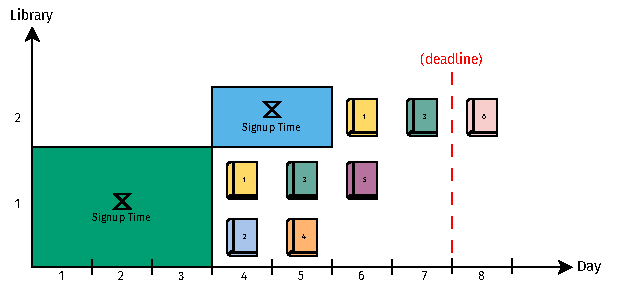
\includegraphics[width=0.8\textwidth,keepaspectratio]{../assets/bs/bs-example-slides.pdf}
  \end{figure}
  \begin{table}
    \begin{tabular}{cc}
      \begin{minipage}{0.5\textwidth}
        \begin{table}[ht]
          \centering
          \begin{tabular}{ccccccc}
            \toprule
            \textbf{Book}  & 1          & 2          & 3          & 4          & 5          & 6 \\ \midrule
            \textbf{Score} & \textbf{3} & \textbf{1} & \textbf{5} & \textbf{4} & \textbf{7} & 1 \\
            \bottomrule
          \end{tabular}
        \end{table}
      \end{minipage}
       &
      \begin{minipage}[b]{0.5\textwidth}
        \centering
        \begin{equation*}
          f(x) = 3 + 1 + 5 + 4 + 7 = 20
        \end{equation*}
      \end{minipage}
    \end{tabular}
    \caption{Book Scores \& Objective Value}
  \end{table}
\end{frame}

\begin{frame}{Modeling --- Problem, Solution and Component}
  The~\alert{problem} is characterized by the set of all libraries available, along with
  their sign-up times, book shipping rate, and list of books that can be shipped,
  the scores for all the books, and the deadline.

  A~\alert{solution} is characterized by a collection of assignments of books
  to libraries and the order in which libraries are scanned.

  A~\alert{component} is characterized by a tuple containing a book and a library or
  a tuple containing two libraries (denoting the sign-up order).
\end{frame}

\begin{frame}{Modeling --- Construction Rules}
  Two component enumeration strategies were considered:
  \begin{itemize}
    \item \textbf{Standard:} Enumerate all the books that can be scanned by all signed-up libraries
          as well as all libraries that can be signed-up until the deadline.
    \item \textbf{Sequential:} Enumerate only the books of the last signed-up library and all the libraries
          that can still be signed-up.
  \end{itemize}
\end{frame}

\begin{frame}{Modeling -- Upper Bound}
  The upper bounds were devised for this problem are as follows:
  \begin{enumerate}
    \item \textbf{Individual Library Knapsacks:} In this approach, we treat the
          number of books each library can scan before the deadline as an individual
          knapsack. The bound value for each library is calculated as the sum of
          scores from the best books that are yet to be scanned. The
          global upper bound is then determined by summing up the bound values for
          each library.

    \item \textbf{Combined Knapsack for All Libraries:} Consider a single
          knapsack representing the total number of books that can be scanned by
          all libraries combined until the deadline.
  \end{enumerate}
\end{frame}

\begin{frame}{Modeling -- Local Moves}
  The~\alert{local moves} considered for this problem are:

  \begin{enumerate}
    \item \textbf{Adding a book} to the set of books to be scanned by a given library.
    \item \textbf{Removing a book} from the set of books that were going to be scanned by a library.
    \item \textbf{Swapping books between libraries}.
    \item \textbf{Removing a book} from the list of books to be scanned by a library and
          \textbf{adding that book to another library}. If possible, ~\textbf{replace the removed book} in
          the first library~\textbf{with another one} that is available there.
  \end{enumerate}
\end{frame}

\begin{frame}{Modeling --- Two-Phase Approach}
  Use a meta-heuristic to choose an order for the libraries and solve the book assignment problem optimally.

  Notably, the assignment problem can be modeled as bipartite graph and solved with any
  \textbf{min cost max-flow} solver.

  \begin{figure}[h]
    \centering
    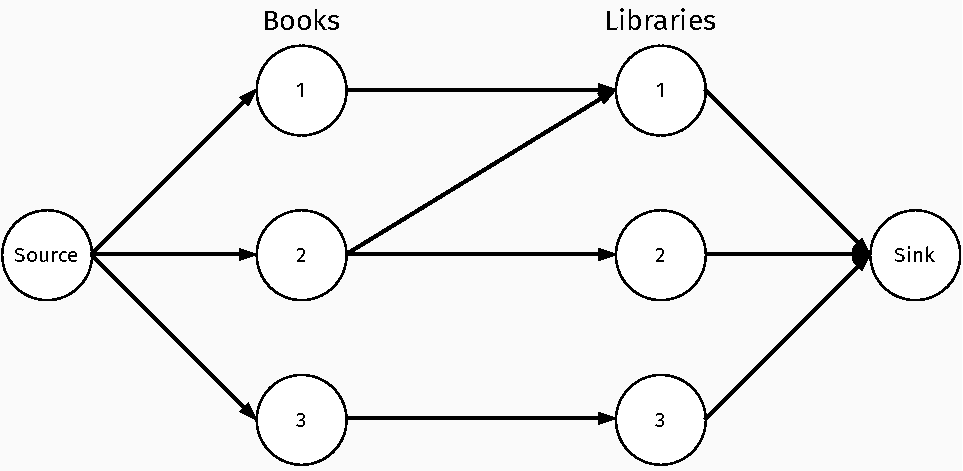
\includegraphics[width=0.8\textwidth,keepaspectratio]{../assets/bs/bs-graph-slides.pdf}
    \caption{Assignment Problem Modeled as a Bipartite Graph}
  \end{figure}
\end{frame}

\begin{frame}{Modeling --- Two-Phase Approach Local Moves}
  After the book assignment the solution can be further improved through
  the following~\alert{local moves}:
  \begin{enumerate}
    \item \textbf{Reverse the sign-up order} between two libraries.
    \item \textbf{Change the positions of two libraries} in the order adjusting the
          sign-up times of every library in between.
    \item \textbf{Select one library to remove and add another library} that is not
          currently considered in that position, if possible.
  \end{enumerate}
\end{frame}

\begin{frame}{Results}
  The best objective values for the five instance of this problem were obtained using the
  \textbf{two-phase} approach, as illustrated in the table below:

  \begin{table}[ht]
    \centering
    \begin{tabular}{@{\extracolsep{4pt}}lcc@{\extracolsep{4pt}}}
      \toprule
      Instance                           & Objective Value & Best Known Objective Value \\ \midrule
      \textquote{Read On}                & \num{5822900}   & \num{5822900}              \\
      \textquote{Incunabula}             & \num{5689822}   & \num{5690888}              \\
      \textquote{Tough Choices}          & \num{5028530}   & \num{5107113}              \\
      \textquote{So many books}          & \num{5208455}   & \num{5237345}              \\
      \textquote{Libraries of the world} & \num{5328034}   & \num{5348248}              \\
      \bottomrule
    \end{tabular}
    \caption{Book Scanning Best Results}
  \end{table}

  Remarkably, this objective value would have placed us in~\textbf{33rd}
  place~(out of 10716 teams) on the competition leaderboard.
\end{frame}

\subsection{Iterated Local Search}
\label{subsec:ils}
% Constructive Search Procedure (algorithm2e pseudocode)

\KwIn{Solution ($s$), Kick Strength ($k$), Objective Function ($f$)}
\KwOut{Solution ($s$).}

\SetKwFunction{Perturb}{\texttt{Perturb}}
\SetKwFunction{LocalSearch}{\texttt{LocalSearch}}

\While{\texttt{stopping criteria not met}}{
  $s'$ $\gets$ \LocalSearch{$s$}\;
  $s'$ $\gets$ \Perturb{$s', k$}\;
  \If{$f(s') > f(s$)}{
    $s$ $\gets$ $s'$\;
  }
}
\Return{$s$}